\section{Durchführung}
\label{sec:Durchführung}
Der Versuchsaufbau wird in der Abbildung \ref{fig:Aufbau} dargestellt.
\begin{figure}[H]
    \centering
    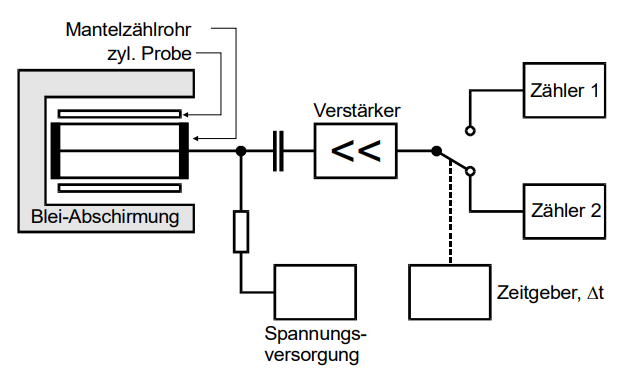
\includegraphics[scale=0.5]{content/Aufbau.png}
    \caption{Darstellung des Verwendeten versuchsaufbau.}
    \label{fig:Aufbau}
\end{figure}
Durch die Blei-Abschirmung wir der Einfluss der Umgebungsradioaktivität gering gehalten.
Mithife eines Geiger-Müller-Zählrohr, welches sich in der Abschirmung befindet, werden die emittierten $\beta$- und $\gamma$-Teilchen der jeweiligen Proben aufgenommen.
Die Anzeige der Zähler schaltet sich automatisch periodisch um, so dass die Zählergebnis abgelesen werden kann und die Messung ohne Unterbrechung
weiter laufen kann.\\

Zu Beginn des Versuchs wird der Nulleffekt $N_u$ gemessen.
Dieser entsteht durch die natürliche Radioaktivität und der Höhenaktivität.
Bei dieser Messung befindetet sich keine Probe in der Abschirmung.
Es wird in einem gesamten Zeitraum von mindestens $\qty{500}{s}$ bis $\qty{600}{s}$ gemessen.\\

Es wird nun zur Bestimmung der Halbwertszeit von Silberisotope das Silberpräparat aus dem Behälter, der in der Abbildung \ref{fig:QN} dargestellt wird geholt
und in die Blei-Abschirmung gebracht.
Dabei ist darauf zu achten, dass dies so schnell wie möglich passiert, damit die sehr schnell Ablaufenden einfach Zerfälle gemessen werden können.
Die Messung wird zweimal durchgeführt.
In der ersten Messung wurde in einem Zeitintervall von $\qty{10}{s}$ und bei der zweiten Messung $\qty{8}{s}$ gemessen.
Die gesamte Messzeit beträgt jeweil $\qty{7}{min}$.
Nach der ersten Messung wird das Silber-Präparat wieder in dem Behälter augeladen.
Die Aufladungszeit beträgt dabei $\qty{15}{min}$.\\

Bei der nächsten Messung wird Vanadium verwendet.
Dies wird auch aus dem Behälter aus Abbildung \ref{fig:QN} geholt.
Die Messung wird in einem Intervall von $\qty{35}{s}$ durchgeführt.
Der gesamte Zeitraum der Messung beträgt $\qty{25}{min}$. 

